\documentclass[border=3pt,tikz]{standalone}
\usepackage{amsmath}
\usetikzlibrary{arrows.meta}
\usetikzlibrary{calc}
\begin{document}
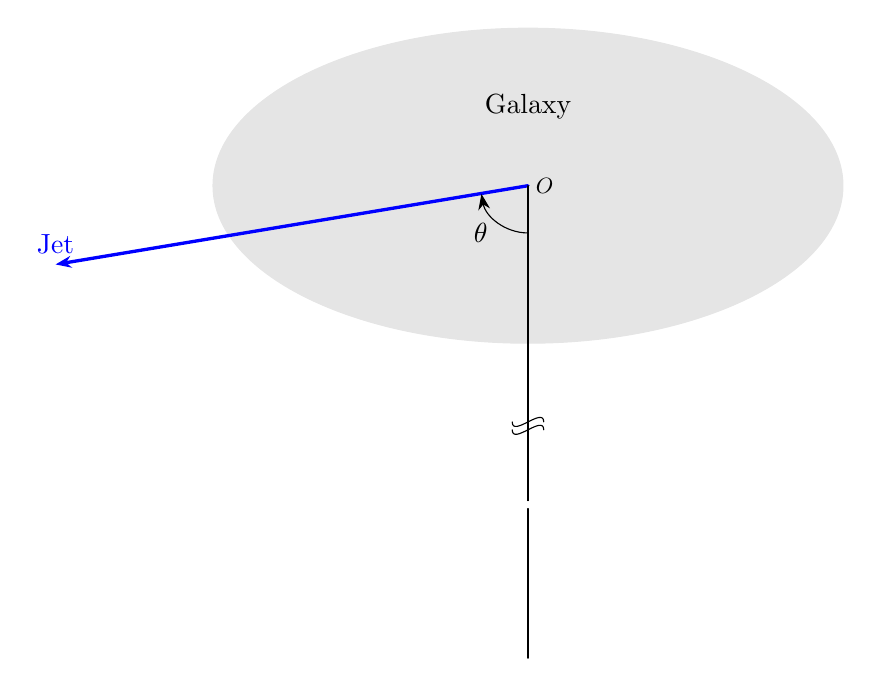
\begin{tikzpicture}[line cap=round, scale = 2]


    \draw [gray!20, fill=gray!20] (0,0) ellipse (2 and 1);
    \node[right, scale=0.8] at (0, 0) {$O$};
    \node [black, scale=1] at (0, 0.5) {Galaxy};
    \draw [very thick, blue, -{Stealth[length=2mm]}] (0, 0) -- (-3, -0.5) node[above, scale=1] {Jet};
    \draw [] (0, -3) -- (0, -2.05);
    \draw [] (0, -2) -- (0, -0);
    
    \draw (-0.1,-1.5) .. controls + (0,-0.1) and + (0,0.1) ..  ++ (0.2, 0)    ++ (0,-0.2);
    \draw (-0.1,-1.55) .. controls + (0,-0.1) and + (0,0.1) ..  ++ (0.2, 0)    ++ (0,-0.2);
    
    \draw[-{Stealth[length=2mm]}] (0, -0.3) arc (270:190:0.3);
    \node [] at (-0.3, -0.3) {$\theta$}; 
    
    \begin{scope}[shift={(4,0)}]
    \end{scope}
    
    \end{tikzpicture}
\end{document}